% Created by tikzDevice version 0.12 on 2018-12-03 20:41:36
% !TEX encoding = UTF-8 Unicode
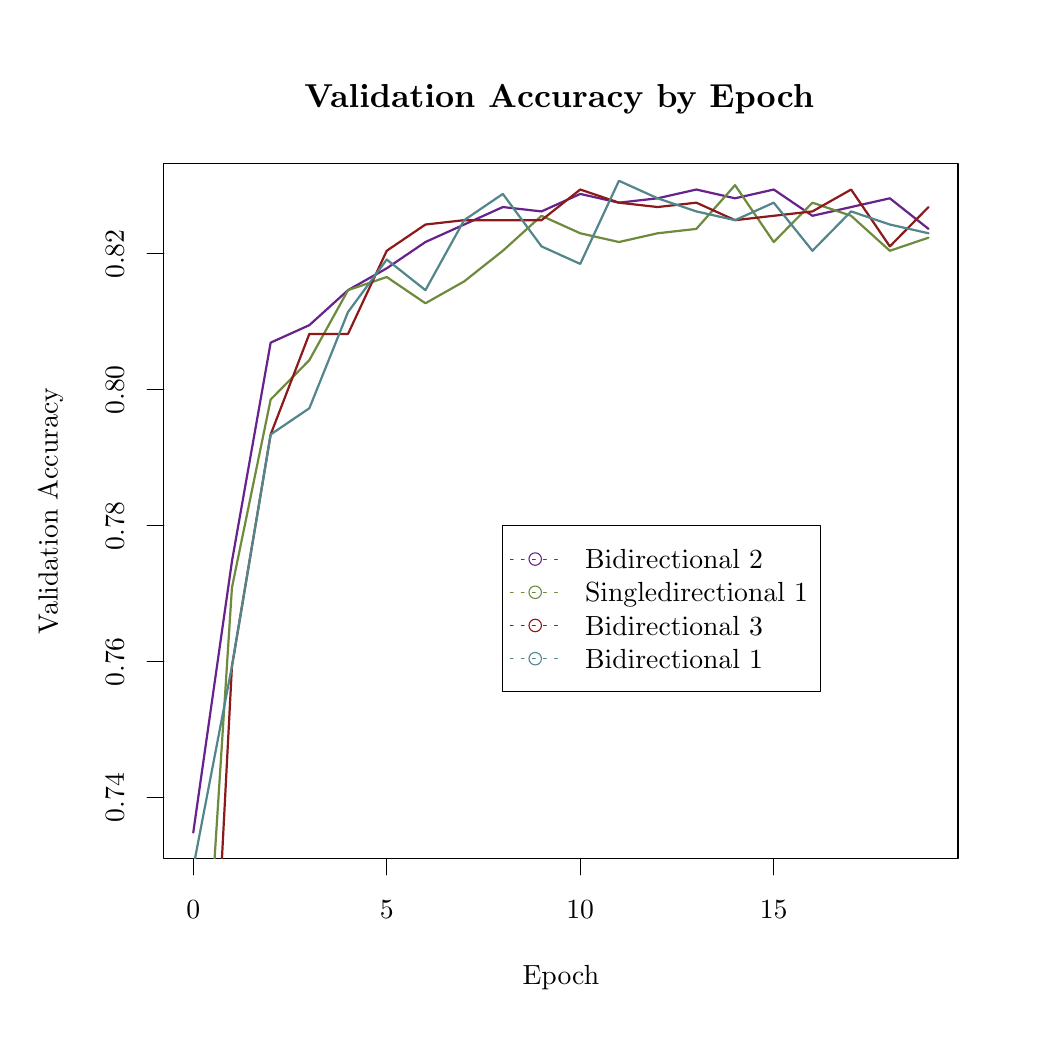
\begin{tikzpicture}[x=1pt,y=1pt]
\definecolor{fillColor}{RGB}{255,255,255}
\path[use as bounding box,fill=fillColor,fill opacity=0.00] (0,0) rectangle (361.35,361.35);
\begin{scope}
\path[clip] ( 49.20, 61.20) rectangle (336.15,312.15);
\definecolor{drawColor}{RGB}{255,255,255}

\path[draw=drawColor,line width= 0.8pt,line join=round,line cap=round] ( 59.83, 70.49) circle (  2.25);

\path[draw=drawColor,line width= 0.8pt,line join=round,line cap=round] ( 73.81,168.50) circle (  2.25);

\path[draw=drawColor,line width= 0.8pt,line join=round,line cap=round] ( 87.80,247.53) circle (  2.25);

\path[draw=drawColor,line width= 0.8pt,line join=round,line cap=round] (101.78,253.85) circle (  2.25);

\path[draw=drawColor,line width= 0.8pt,line join=round,line cap=round] (115.76,266.50) circle (  2.25);

\path[draw=drawColor,line width= 0.8pt,line join=round,line cap=round] (129.75,274.40) circle (  2.25);

\path[draw=drawColor,line width= 0.8pt,line join=round,line cap=round] (143.73,283.89) circle (  2.25);

\path[draw=drawColor,line width= 0.8pt,line join=round,line cap=round] (157.72,290.21) circle (  2.25);

\path[draw=drawColor,line width= 0.8pt,line join=round,line cap=round] (171.70,296.53) circle (  2.25);

\path[draw=drawColor,line width= 0.8pt,line join=round,line cap=round] (185.68,294.95) circle (  2.25);

\path[draw=drawColor,line width= 0.8pt,line join=round,line cap=round] (199.67,301.27) circle (  2.25);

\path[draw=drawColor,line width= 0.8pt,line join=round,line cap=round] (213.65,298.11) circle (  2.25);

\path[draw=drawColor,line width= 0.8pt,line join=round,line cap=round] (227.63,299.69) circle (  2.25);

\path[draw=drawColor,line width= 0.8pt,line join=round,line cap=round] (241.62,302.86) circle (  2.25);

\path[draw=drawColor,line width= 0.8pt,line join=round,line cap=round] (255.60,299.69) circle (  2.25);

\path[draw=drawColor,line width= 0.8pt,line join=round,line cap=round] (269.59,302.86) circle (  2.25);

\path[draw=drawColor,line width= 0.8pt,line join=round,line cap=round] (283.57,293.37) circle (  2.25);

\path[draw=drawColor,line width= 0.8pt,line join=round,line cap=round] (297.55,296.53) circle (  2.25);

\path[draw=drawColor,line width= 0.8pt,line join=round,line cap=round] (311.54,299.69) circle (  2.25);

\path[draw=drawColor,line width= 0.8pt,line join=round,line cap=round] (325.52,288.63) circle (  2.25);
\end{scope}
\begin{scope}
\path[clip] (  0.00,  0.00) rectangle (361.35,361.35);
\definecolor{drawColor}{RGB}{0,0,0}

\path[draw=drawColor,line width= 0.4pt,line join=round,line cap=round] ( 59.83, 61.20) -- (269.59, 61.20);

\path[draw=drawColor,line width= 0.4pt,line join=round,line cap=round] ( 59.83, 61.20) -- ( 59.83, 55.20);

\path[draw=drawColor,line width= 0.4pt,line join=round,line cap=round] (129.75, 61.20) -- (129.75, 55.20);

\path[draw=drawColor,line width= 0.4pt,line join=round,line cap=round] (199.67, 61.20) -- (199.67, 55.20);

\path[draw=drawColor,line width= 0.4pt,line join=round,line cap=round] (269.59, 61.20) -- (269.59, 55.20);

\node[text=drawColor,anchor=base,inner sep=0pt, outer sep=0pt, scale=  1.00] at ( 59.83, 39.60) {0};

\node[text=drawColor,anchor=base,inner sep=0pt, outer sep=0pt, scale=  1.00] at (129.75, 39.60) {5};

\node[text=drawColor,anchor=base,inner sep=0pt, outer sep=0pt, scale=  1.00] at (199.67, 39.60) {10};

\node[text=drawColor,anchor=base,inner sep=0pt, outer sep=0pt, scale=  1.00] at (269.59, 39.60) {15};

\path[draw=drawColor,line width= 0.4pt,line join=round,line cap=round] ( 49.20, 83.08) -- ( 49.20,279.59);

\path[draw=drawColor,line width= 0.4pt,line join=round,line cap=round] ( 49.20, 83.08) -- ( 43.20, 83.08);

\path[draw=drawColor,line width= 0.4pt,line join=round,line cap=round] ( 49.20,132.20) -- ( 43.20,132.20);

\path[draw=drawColor,line width= 0.4pt,line join=round,line cap=round] ( 49.20,181.33) -- ( 43.20,181.33);

\path[draw=drawColor,line width= 0.4pt,line join=round,line cap=round] ( 49.20,230.46) -- ( 43.20,230.46);

\path[draw=drawColor,line width= 0.4pt,line join=round,line cap=round] ( 49.20,279.59) -- ( 43.20,279.59);

\node[text=drawColor,rotate= 90.00,anchor=base,inner sep=0pt, outer sep=0pt, scale=  1.00] at ( 34.80, 83.08) {0.74};

\node[text=drawColor,rotate= 90.00,anchor=base,inner sep=0pt, outer sep=0pt, scale=  1.00] at ( 34.80,132.20) {0.76};

\node[text=drawColor,rotate= 90.00,anchor=base,inner sep=0pt, outer sep=0pt, scale=  1.00] at ( 34.80,181.33) {0.78};

\node[text=drawColor,rotate= 90.00,anchor=base,inner sep=0pt, outer sep=0pt, scale=  1.00] at ( 34.80,230.46) {0.80};

\node[text=drawColor,rotate= 90.00,anchor=base,inner sep=0pt, outer sep=0pt, scale=  1.00] at ( 34.80,279.59) {0.82};

\path[draw=drawColor,line width= 0.4pt,line join=round,line cap=round] ( 49.20, 61.20) --
	(336.15, 61.20) --
	(336.15,312.15) --
	( 49.20,312.15) --
	( 49.20, 61.20);
\end{scope}
\begin{scope}
\path[clip] (  0.00,  0.00) rectangle (361.35,361.35);
\definecolor{drawColor}{RGB}{0,0,0}

\node[text=drawColor,anchor=base west,inner sep=0pt, outer sep=0pt, scale=  1.20] at ( 100.00,332.61) {\bfseries Validation Accuracy by Epoch};

\node[text=drawColor,anchor=base,inner sep=0pt, outer sep=0pt, scale=  1.00] at (192.68, 15.60) {Epoch};

\node[text=drawColor,rotate= 90.00,anchor=base,inner sep=0pt, outer sep=0pt, scale=  1.00] at ( 10.80,186.68) {Validation Accuracy};
\end{scope}
\begin{scope}
\path[clip] ( 49.20, 61.20) rectangle (336.15,312.15);
\definecolor{drawColor}{RGB}{104,34,139}

\path[draw=drawColor,line width= 0.8pt,line join=round,line cap=round] ( 59.83, 70.49) --
	( 73.81,168.50) --
	( 87.80,247.53) --
	(101.78,253.85) --
	(115.76,266.50) --
	(129.75,274.40) --
	(143.73,283.89) --
	(157.72,290.21) --
	(171.70,296.53) --
	(185.68,294.95) --
	(199.67,301.27) --
	(213.65,298.11) --
	(227.63,299.69) --
	(241.62,302.86) --
	(255.60,299.69) --
	(269.59,302.86) --
	(283.57,293.37) --
	(297.55,296.53) --
	(311.54,299.69) --
	(325.52,288.63);
\definecolor{drawColor}{RGB}{110,139,61}

\path[draw=drawColor,line width= 0.8pt,line join=round,line cap=round] ( 63.62,  0.00) --
	( 73.81,159.01) --
	( 87.80,226.98) --
	(101.78,241.21) --
	(115.76,266.50) --
	(129.75,271.24) --
	(143.73,261.76) --
	(157.72,269.66) --
	(171.70,280.73) --
	(185.68,293.37) --
	(199.67,287.05) --
	(213.65,283.89) --
	(227.63,287.05) --
	(241.62,288.63) --
	(255.60,304.44) --
	(269.59,283.89) --
	(283.57,298.11) --
	(297.55,293.37) --
	(311.54,280.73) --
	(325.52,285.47);
\definecolor{drawColor}{RGB}{139,26,26}

\path[draw=drawColor,line width= 0.8pt,line join=round,line cap=round] ( 67.02,  0.00) --
	( 73.81,130.56) --
	( 87.80,214.34) --
	(101.78,250.69) --
	(115.76,250.69) --
	(129.75,280.73) --
	(143.73,290.21) --
	(157.72,291.79) --
	(171.70,291.79) --
	(185.68,291.79) --
	(199.67,302.86) --
	(213.65,298.11) --
	(227.63,296.53) --
	(241.62,298.11) --
	(255.60,291.79) --
	(269.59,293.37) --
	(283.57,294.95) --
	(297.55,302.86) --
	(311.54,282.31) --
	(325.52,296.53);
\definecolor{drawColor}{RGB}{83,134,139}

\path[draw=drawColor,line width= 0.8pt,line join=round,line cap=round] ( 59.83, 57.85) --
	( 73.81,130.56) --
	( 87.80,214.34) --
	(101.78,223.82) --
	(115.76,258.60) --
	(129.75,277.56) --
	(143.73,266.50) --
	(157.72,291.79) --
	(171.70,301.27) --
	(185.68,282.31) --
	(199.67,275.98) --
	(213.65,306.02) --
	(227.63,299.69) --
	(241.62,294.95) --
	(255.60,291.79) --
	(269.59,298.11) --
	(283.57,280.73) --
	(297.55,294.95) --
	(311.54,290.21) --
	(325.52,287.05);
\definecolor{drawColor}{RGB}{0,0,0}

\path[draw=drawColor,line width= 0.4pt,line join=round,line cap=round] (171.70,181.33) rectangle (286.46,121.33);
\definecolor{drawColor}{RGB}{104,34,139}

\path[draw=drawColor,line width= 0.4pt,dash pattern=on 1pt off 3pt ,line join=round,line cap=round] (174.40,169.33) -- (192.40,169.33);
\definecolor{drawColor}{RGB}{110,139,61}

\path[draw=drawColor,line width= 0.4pt,dash pattern=on 1pt off 3pt ,line join=round,line cap=round] (174.40,157.33) -- (192.40,157.33);
\definecolor{drawColor}{RGB}{139,26,26}

\path[draw=drawColor,line width= 0.4pt,dash pattern=on 1pt off 3pt ,line join=round,line cap=round] (174.40,145.33) -- (192.40,145.33);
\definecolor{drawColor}{RGB}{83,134,139}

\path[draw=drawColor,line width= 0.4pt,dash pattern=on 1pt off 3pt ,line join=round,line cap=round] (174.40,133.33) -- (192.40,133.33);
\definecolor{drawColor}{RGB}{104,34,139}

\path[draw=drawColor,line width= 0.4pt,line join=round,line cap=round] (183.40,169.33) circle (  2.25);
\definecolor{drawColor}{RGB}{110,139,61}

\path[draw=drawColor,line width= 0.4pt,line join=round,line cap=round] (183.40,157.33) circle (  2.25);
\definecolor{drawColor}{RGB}{139,26,26}

\path[draw=drawColor,line width= 0.4pt,line join=round,line cap=round] (183.40,145.33) circle (  2.25);
\definecolor{drawColor}{RGB}{83,134,139}

\path[draw=drawColor,line width= 0.4pt,line join=round,line cap=round] (183.40,133.33) circle (  2.25);
\definecolor{drawColor}{RGB}{0,0,0}

\node[text=drawColor,anchor=base west,inner sep=0pt, outer sep=0pt, scale=  1.00] at (201.40,165.89) {Bidirectional 2};

\node[text=drawColor,anchor=base west,inner sep=0pt, outer sep=0pt, scale=  1.00] at (201.40,153.89) {Singledirectional 1};

\node[text=drawColor,anchor=base west,inner sep=0pt, outer sep=0pt, scale=  1.00] at (201.40,141.89) {Bidirectional 3};

\node[text=drawColor,anchor=base west,inner sep=0pt, outer sep=0pt, scale=  1.00] at (201.40,129.89) {Bidirectional 1};
\end{scope}
\end{tikzpicture}
